\documentclass[11pt]{article}
\usepackage[a4paper,margin=24mm]{geometry}
\usepackage{amsmath,amssymb,mathtools,amsthm,tikz}
\usepackage[hidelinks,hypertexnames=false]{hyperref}\usepackage{xurl}
\usetikzlibrary{arrows.meta,positioning}
\setlength{\emergencystretch}{3em}
\title{The original inverse-sector quotient: shifted source, heat localization and covariance-angle control}
\author{Split-Zero research programme}\date{21 September 2026}
\begin{document}\maketitle
The received continuation supplies an explicit quotient of the original
observation complex by its controlled inverse-power sector. This note
proves the analytic receiving estimates in its original metrics and adds
a rank-sensitive bound for the angle change under the complete source
covariance. It also identifies exactly the coefficient already called
$C_\partial$ in the older endpoint work. The full received argument and
its independent finite verification accompany this note.

\section{Objects, guards and the original coefficient}
Keep $0<\delta<1/2$, $\gamma>2$, $k\equiv1\pmod4$,
$q=(k+1)^2$, the original full polynomial $Q_k(y)$,
$E=\mathbb C[y]/(Q_k)$, $M[p]=[yp]$, and the four cutoffs
$N=q-1,q,2q-1,2q$. The physical coordinate is $S=k/2+iy$.
The source is $\mu_k=w_h^{*k}$ and $G_N$ is its attained metric.
Keep the original onto observation $\Lambda:E\to B$, its full kernel
$K$, and its fixed coefficient frame $I_K$. On the proved five-orbit
period domain $m=\dim K=8k-16$; no larger period domain is asserted.

For $1\le r<q$ put $U_rd=\sum_{j=1}^rd_j[y^{-j}]$, $V_r=\operatorname{im}U_r$.
Use every finite guard of IVO1--26 and IFH1--21 \cite{IFH,IVO}.
In particular, on the eventual regime $r\log(q+2)=o(q)$,
\[
H^B_{r,N}\succeq e^{-\varepsilon_{k,r}}H^E_{r,N},\qquad
\varepsilon_{k,r}=O_{h,A}((k+Jr)\log(q+Jr+2))=o(q).
\tag{IQR1}
\]
Here $H^E=U_r^*G_NU_r$, $H^B=U_r^*\Lambda^*Q_{B,N}\Lambda U_r$
and $Q_{B,N}=(\Lambda G_N^{-1}\Lambda^*)^{-1}$.
The exact positive finite IVO factor may replace the exponential bound.

The coefficient in IFH10 is exactly the earlier outer coefficient.
Here is the complete dictionary, retaining its scale.
At the EIQ potential $\pi\sqrt x-2\log x$, let $u,v$ be the actual
positive square-root endpoints and write
\[
uK(\kappa)=2,\quad vE(\kappa)=4,\quad a=u/v,\quad
\kappa^2=1-a^2,\quad w=(u+v)/2,\quad z=uv,\quad c=(v^2-u^2)/4.
\]
ECL1--17 \cite{ECL} proves
$L=\int\log x\,d\rho_1=6\log w-2\log z-2$ and
$C_\partial=4\log(4/\pi)+8\log w-4\log z-2\log c$.
The retained profile has $\psi(0)=\log(4/\pi)$, and S2 gives
\[
\psi(1)=\log\frac{\kappa(1+a)}{E(\kappa)^2}
       =\log\frac{w\sqrt c}{4},\qquad
J(1)=2(\log2-1)-L/2.
\]
The middle equality follows from $v=4/E$, $w=v(1+a)/2$ and
$\sqrt c=v\kappa/2$. Substitution, with every constant retained, proves
\[
\begin{split}
\mathfrak C&=4[\psi(0)-\psi(1)-J(1)-1]\\
 &=4\log(4/\pi)-4\log w-2\log c+4+2L\\
 &=4\log(4/\pi)+8\log w-4\log z-2\log c=C_\partial .
\end{split}\tag{IQR2}
\]
Thus the already reproduced interval
$1.353893<C_\partial<1.354751$ applies to this same older coefficient.
No numerical approximation is used to prove its identity.

\section{Full shifted polynomial sources and their finite errors}
The original quotient coordinates and attained metric are
\[
\pi_r[p]=\mathscr D^r\operatorname{rem}_{Q_k}(y^rp),\qquad
\overline G_{r,N}=(\pi_rG_N^{-1}\pi_r^*)^{-1},\qquad
\widehat H_{K,r,N}=(\pi_rI_K)^*\overline G_{r,N}(\pi_rI_K).
\]
The finite Schur identity in the supplied equations (3)--(9) yields
\[
0\le\delta_{r,N}:=\log\det H_{K,N}-\log\det\widehat H_{K,r,N}
\le\min(m,r)\varepsilon_{k,r}=:\mathcal L_{k,r}.
\tag{IQR3}
\]
All ranks can be replaced by the actual cross-Gram rank.

Let $\mathcal P_L$ be the original physical-$y$ polynomial space with
Gram $H_L^{\rm src}$ for $\mu_k$. In $\mathcal P_{N+r}$ keep the full
column matrix
\[
R_{r,N}=[1,y,\ldots,y^{r-1},Q_k,yQ_k,\ldots,y^{N+r-q}Q_k],
\qquad E_{r,N}=y^rI_K .
\]
The last equality uses degree-below-$q$ representatives of $I_K$.
The columns of $R_{r,N}$ are independent: a relation between them
would make a degree-below-$r<q$ polynomial divisible by $Q_k$.
Their Gram is therefore positive. Completing the full quadratic
minimum gives
\[
H^{\rm sh}_{r,N}=E^*H^{\rm src}_{N+r}E
-E^*H^{\rm src}_{N+r}R(R^*H^{\rm src}_{N+r}R)^{-1}
 R^*H^{\rm src}_{N+r}E .
\tag{IQR4}
\]
This is the metric of $M^rI_K$ in $E/\mathcal P_{<r}$ attained from
the cutoff $N+r$. Multiplication by $M^r$ identifies $E/V_r$
with $E/\mathcal P_{<r}$, since $M^rV_r=\mathcal P_{<r}$.
It sends $\pi_r I_K$ to exactly the classes displayed in IQR4.

Put $n_L=\lceil(L+2)/2\rceil$,
$a_L^\Gamma=\sqrt{n_L(n_L+1)}(1+\sqrt{L+1})$ and
\[
\mathfrak B_{r,L}=\sqrt{u_k/\ell_{k,L}}(a_L^\Gamma)^r,\qquad
\mathfrak A_{r,N}=\prod_{j=0}^{r-1}
 C_{\rm mult}(h)[2(N+j)+\lfloor k/3\rfloor].
\]
S12--16 \cite{Smallest} proves $\|\mathscr D p\|_\sigma\le
a_L^\Gamma\|p\|_\sigma$ for every $\deg p\le L$.
Applying this $r$ times in the same Gamma space and using NG2
only before and after gives
$\|\mathscr D^rp\|_{\mu_k}\le\mathfrak B_{r,L}\|p\|_{\mu_k}$.
The intermediate degree decreases; $a_L^\Gamma$ bounds every step.
NG3 \cite{NG} gives the displayed $\mathfrak A$ for multiplication
by $y^r$, including the entire outgoing degree at every step.

For the forward quotient bound multiply the actual minimum source
representative by $y^r$. For the inverse choose the complete minimum
representative in the target and apply $\mathscr D^r$; the discarded
Taylor polynomial belongs to the exact target relation $\mathcal P_{<r}$.
These are admissible lifts of the inverse isomorphisms, so
\[
\mathfrak B_{r,N+r}^{-2}\widehat H_{K,r,N}
\preceq H^{\rm sh}_{r,N}
\preceq\mathfrak A_{r,N}^2\widehat H_{K,r,N}.
\tag{IQR5}
\]
In particular, with $\log^+x=\max(0,\log x)$, an explicit error is
\[
\begin{split}
\left|\mathcal R\log\det H^{\rm sh}_{r,N}
      -\mathcal R\log\det H_{K,N}\right|
&\le2\mathcal L_{k,r}\\
&\quad+2m\sum_N
 \max\{\log^+\mathfrak A_{r,N},\log^+\mathfrak B_{r,N+r}\}
=o(kq).
\end{split}\tag{IQR6}
\]
Indeed each logarithmic comparison in IQR5 lies between
$-2m\log\mathfrak B$ and $2m\log\mathfrak A$;
IQR3 contributes at most $2\mathcal L$ under two positive and
two negative signs. NG2--3 gives
$\log^+\mathfrak A+\log^+\mathfrak B=O_h(k+r\log q)$
for these full degrees $N+r=O(q)$. This is $o(q)$.
No shifted cutoff has been relabelled as an unshifted one.

For $1\le s\le r$, let $Z=(I-P_{V_r,N})I_K$.
Its original Gram is $\widehat H_{K,r,N}$.
The exact Taylor-division inverse identity kills its rank-$s$
remainder after projection perpendicular to $V_r$, proving
$\|M^sx\|\ge\mathfrak B_{s,N}^{-1}\|x\|$ for $x\perp V_r$.
The original decomposition $M=C_N+R_N$ has rank $R_N=1$,
$\|C_N\|\le B_hq$, and $\|R_N\|=\epsilon_N$ \cite{Profile}.
The min--max principle on $\ker R_N$ gives
$\sigma_j(M)\le B_hq$ for $j\ge2$, and the triangle inequality
bounds $\sigma_1(M)\le\epsilon_N+B_hq$.
Applying the $m$th exterior power to $M^s$ therefore proves
\[
\begin{split}
-2m\log\mathfrak B_{s,N}
&\le \log\frac{\det((M^sZ)^*G_NM^sZ)}{\det\widehat H_{K,r,N}}\\
&\le2s\log(\epsilon_N+B_hq)+2s(m-1)\log(B_hq).
\end{split}\tag{IQR7}
\]
Here the product of the largest $m$ singular values is the norm of
the $m$th exterior map; this follows by exteriorizing a singular-value
decomposition. Its norm is submultiplicative under composition.
Since $\log^+\epsilon_N=O_h(q)$, IQR3 and IQR7 preserve the
original $kq$ coefficient for $s=o(k)$.
The original source order, not a truncated multiplication, supplies this bound.

\section{Quadratic residual heat and the actual eigenclass stack}
All adjoints and projections in this section use $G_N$.
For $r\ge1$, let $W^E=P_{B,N}V_r$ and
$P_{\rm rem}=P_{B,N}-P_{W^E}$.
The inclusion $W^E\subset K^\perp$ makes this an orthogonal projection.
Its image is $(K+V_r)^\perp$: an element of $K^\perp$ pairs
with $P_BV_r$ exactly as it pairs with $V_r$.
The fixed class $u=-Q_k(0)[y^{-1}]$ lies in $V_r$.
Thus $P_{\rm rem}u=0$.

Let $a_N$ be a unit smallest right singular vector, and retain the
actual finite LS guard $E_N>2D_N$ and $\eta_N=D_N/(E_N-D_N)$.
LS4 gives $\|(I-P_u)a_N\|\le\eta_N$, and hence
$\|P_{\rm rem}a_N\|^2\le\eta_N^2$. In the full orthonormal singular
basis the other eigenvalues of $M^\dagger M$ are at least $D_N^{-2}$.
Every corresponding projection weight lies in $[0,1]$. Therefore
\[
0\le\operatorname{Tr}(P_{\rm rem}e^{-\tau M^\dagger M})
\le \eta_N^2e^{-\tau s_N^2}+(q-1)e^{-\tau/D_N^2}.
\tag{IQR8}
\]
This proves the quadratic angle error without discarding a heat direction.

Write $\theta_N=\|P_Bu\|^2/\|u\|^2$ and use the exact IFH11
relative error $r_N(\tau)$. When $r_N(\tau)<1$, its positive lower
bound for the original measured heat gives the finite fraction estimate
\[
0\le
\frac{\operatorname{Tr}(P_{\rm rem}e^{-\tau M^\dagger M})}
     {\operatorname{Tr}(P_Be^{-\tau M^\dagger M})}
\le
\frac{\eta_N^2+(q-1)e^{-\tau(D_N^{-2}-s_N^2)}}
     {\theta_N(1-r_N(\tau))}.
\tag{IQR9}
\]
The right side tends to zero at the unchanged common time
$\tau_k^*=\exp\{2q[\log(q/k)-1-I(\delta,\gamma)/2]\}$,
including the two high cutoffs whose surviving mass is very small.
In fact $\theta_N\ge e^{-O(k\log q)}$,
$\eta_N=e^{-q\log(q/k)+O_h(q)}$ and
$\tau_k^*(D_N^{-2}-s_N^2)$ grows faster than every power of $q$.
Summing the four nonnegative upper bounds in IQR8 proves
\[
\limsup\frac{\log|\mathcal R\operatorname{Tr}
(P_{\rm rem}e^{-\tau_k^*M^\dagger M})|}
{q\log(q/k)}\le-2,\qquad \log0=-\infty .
\tag{IQR10}
\]
IQR9 also proves that the removed observed sector carries a fraction
tending to one of the full observed heat at every cutoff.

Let $S_r:E/V_r\to E$ be the original minimum section, an isometry
onto $V_r^\perp$. LS2 reads $M^{-1}=B_N-u\varphi_N/Q_k(0)$
with $\|B_N\|\le D_N$. For $x\perp V_r$,
$x=(I-P_{V_r})B_NMx$, so
\[
S_r^\dagger M^\dagger MS_r\succeq D_N^{-2}I.
\tag{IQR11}
\]
This is the full-output square of the rectangular map $MS_r$.
The block resolvent and memory formula IFH16--17 gives its exact
relation to the independently compressed observed action.

For the older NP18 stack, preserve multiplication by the physical
coordinate $S$: $A_S=(k/2)I+iM$. If $e_\lambda$ is the cardinal
$y$-eigenclass, its physical eigenvalue is $\mu=k/2+i\lambda$.
For every integer depth $d\ge0$ used at all four cutoffs,
\[
\left\|(\Lambda,\Lambda A_S,\ldots,\Lambda A_S^d)e_\lambda\right\|^2
=\left(\sum_{j=0}^d|\mu|^{2j}\right)
 \|\Lambda e_\lambda\|_{Q_{B,N}}^2 .
\tag{IQR12}
\]
Each term follows from $A_S^je_\lambda=\mu^je_\lambda$;
the output stack has the direct-sum metric with the full $Q_{B,N}$.
The geometric factor cancels exactly under $\mathcal R$, for growing
as well as fixed $d$. IFH20 bounds the observed fraction
$\beta_N\in[e^{-Ck\log(q+2)},1]$ on the detected-line domain.
Consequently $|\mathcal R\log\beta_N|\le2Ck\log(q+2)=o(q)$.
Together with IQR2, NP19 now has coefficient $C_\partial=\mathfrak C$
on that domain. This is an update to that specific canonical angle term.

\section{Complete source covariance and a new angle bound}
Let the complete actual normal source have Gram $H_Z$ and value
map $F_Z$, with $\ker H_Z\subseteq\ker F_Z$.
Retain its full cross terms in $\Omega=F_ZH_Z^+F_Z^*\succeq0$.
For $t\ge0$ the specified activation gives
$G(t)=(G^{-1}+t\Omega)^{-1}$. At a fixed period $\pi=\pi_r$ is fixed,
so its full quotient is exactly
\[
\overline G(t)=(\pi G^{-1}\pi^*+t\pi\Omega\pi^*)^{-1}.
\tag{IQR13}
\]
No orthogonality between unprocessed source groups is inserted.

Put $C=G^{1/2}\Omega G^{1/2}$ and
$S=\overline G(0)^{1/2}\pi G^{-1/2}$.
Then $SS^*=I$, and the quotient covariance is
$\overline C=SCS^*$.
The min--max characterization gives
$\lambda_j(C)\ge\lambda_j(\overline C)\ge\lambda_{j+r}(C)$
in decreasing order. Apply the increasing functions
$f_t(x)=tx/(1+tx)$ and $g_t(x)=\log(1+tx)$ and sum.
The two sides telescope to at most the top $r$ terms, proving
\[
\begin{gathered}
0\le\operatorname{Tr}f_t(C)-\operatorname{Tr}f_t(\overline C)\le r,\\
0\le\operatorname{Tr}g_t(C)-\operatorname{Tr}g_t(\overline C)
 \le r\log(1+t\|C\|).
\end{gathered}\tag{IQR14}
\]
The complete C7 bound \cite{Mixed} therefore acquires just $r/q$
after division by $q$, for $b\ge0$ and $t=e^{-2bq\log(q/k)}$.
For the H23 scale $t=e^{-2\theta q}$, $\theta\ge0$,
$\log(1+\|C\|)=O_h(q\log(q/k))$ gives an additional $o(q^2)$
when $r\log q=o(q)$. The ensuing original observation removes
another $m$ dimensions and costs at most
$m\log(1+t\|C\|)=o(q^2)$. This proves the received (48)
on its original simple-quartet and period domain, with the same $C_B$.
It does not infer a $kq$ estimate from that $q^2$ result.

There is, however, a sharper angle control for small covariance rank.
Keep the fixed disjoint subspaces $K,V=V_r$ and $S_0=K+V$.
For a subspace $X$ with a fixed full frame $I_X$, write
$P_X(t)=I_X(I_X^*G(t)I_X)^{-1}I_X^*G(t)$.
Use the concatenated frame $[I_K,U_r]$ on $S_0$, and set
\[
\delta(t)=\log\det H_K(t)+\log\det H_V(t)
          -\log\det H_{S_0}(t)\ge0 .
\]
Its nonnegativity and its equality to the source/observed angle loss
follow from the full Schur determinant identity.
Since $G'(t)=-G(t)\Omega G(t)$, cyclicity of trace proves, for $t>0$,
\[
t\delta'(t)=-\operatorname{Tr}(D_t A_t),\quad
D_t=tG(t)^{1/2}\Omega G(t)^{1/2},\quad
A_t=\widetilde P_K(t)+\widetilde P_V(t)-\widetilde P_{S_0}(t),
\tag{IQR15}
\]
where $\widetilde P_X=G(t)^{1/2}P_XG(t)^{-1/2}$ is the exact
Euclidean orthogonal projection corresponding to the original metric.
Thus IQR15 is a proved coordinate identity, with both subspaces moving
under this isometry and the physical subspaces fixed.

Here is the spectrum of $A_t$, including all nontrivial directions.
Take orthonormal frames of the two transformed subspaces and a singular
value decomposition of their cross Gram. Its singular values are
$c_j\in[0,1)$ because the two original subspaces have zero intersection.
For each $c_j>0$ choose paired unit vectors
$e_j\in G(t)^{1/2}K$, $f_j\in G(t)^{1/2}V$
with $\langle e_j,f_j\rangle=c_j$.
In the orthonormal pair $e_j,(f_j-c_je_j)/\sqrt{1-c_j^2}$,
the restriction of $A_t$ is
\[
\begin{pmatrix}
c_j^2&c_j\sqrt{1-c_j^2}\\
c_j\sqrt{1-c_j^2}&-c_j^2
\end{pmatrix}.
\tag{IQR16}
\]
Its characteristic polynomial is $\lambda^2-c_j^2$.
All remaining directions give zero, including directions exterior to
$S_0$. Thus $A_t$ has paired eigenvalues $\pm c_j$, with
$\nu(t)=\operatorname{rank}(I_K^*G(t)U_r)\le\min(m,r)$ pairs.

Set $d_\Omega=\operatorname{rank}\Omega$ and $c=\|C\|$.
The positive operator $D_t$ has rank $d_\Omega$ and norm
$tc/(1+tc)$. To see this exactly, $G(t)\Omega$ is similar to
$(I+tC)^{-1}C$, and $D_t$ is similar to $tG(t)\Omega$.
If $A_t=A_+-A_-$ is its positive/negative spectral decomposition,
then $0\preceq A_\pm\preceq I$ and each has rank $\nu(t)$.
For any positive $D$,
$\operatorname{Tr}(DA_\pm)\le
\min\{\operatorname{rank}D,\nu(t)\}\|D\|$:
use both the bound by $\operatorname{Tr}D$ and the bound by
$\nu(t)\|D\|$. It follows that
\[
\begin{gathered}
|t\delta'(t)|
\le\min(m,r,d_\Omega)\frac{tc}{1+tc},\\
|\delta(t)-\delta(0)|
\le\sum_{j=1}^{\ell}\log(1+t\lambda_j(C))
\le\ell\log(1+tc),\qquad \ell=\min(m,r,d_\Omega).
\end{gathered}
\tag{IQR17}
\]
For the stronger middle bound, diagonalize $D_t$. The diagonal weights
of $A_+$ or $A_-$ in that eigenbasis lie in $[0,1]$ and their sum
is at most $\nu(t)$. Their weighted eigenvalue sum is therefore at most
the sum of the largest $\ell$ eigenvalues of $D_t$; moving weight from
a smaller eigenvalue to a larger one proves this directly.
These eigenvalues are $t\lambda_j(C)/(1+t\lambda_j(C))$.
Integrating proves the displayed spectral sum with its original
covariance eigenvalues retained.
The integral from zero is finite; smoothness of the positive finite
Grams extends the identity to $t=0$. If $c=0$, the path is constant.

This supplies an explicit control of the previously retained correction
in the received equation (49). At each endpoint,
\[
0\le\delta_{r,N}(t_N)\le
\min(m,r)\varepsilon_{k,r}
+\min(m,r,d_{\Omega,N})\log(1+t_N\|C_N\|)=:L_N .
\tag{IQR18}
\]
Hence its four-sign absolute value is at most
$\max\{L_{q-1}+L_q,L_{2q-1}+L_{2q}\}$.
If the actual source covariance has rank bounded by $d_k$,
$d_k\log(q+2)=o(k)$, and its retained logarithmic size is
$O_h(q\log(q+2))$, this proves that the source and observation
quotient still preserves the original activated kernel coefficient
through $o(kq)$ when its starting metric is the canonical $G_N$
to which IQR1 applies. The rank-sensitive finite change IQR17
also holds from an already activated positive metric. In that case its
initial angle is retained; rank alone does not transfer IQR1 to it.
The full joint covariance can have rank $q$; IQR18 retains that rank
and does not assert a $kq$ conclusion for it.

For the actual adjacent scalar source this size is evaluated, not
assumed. Let $\phi_{N+1}=p_{N+1}/\sqrt{\omega_{N+1}}$ be the added
orthonormal source column, and $f_N=[\phi_{N+1}]$ its original value.
Put $\alpha_N=f_N^*G_Nf_N$. The full monic relation norm calculation
H3 \cite{Profile}, with $s=N+1-q$, gives
\[
1+\alpha_N=\frac{\nu_s}{\omega_{N+1}},\qquad
\log(1+\alpha_N)=2q\psi(s/q)+O_h(k\log^2(q+2))=O_h(q).
\tag{IQR22}
\]
Indeed the original minimum representative of $[p_{N+1}]$ is the
difference between its full minimum monic relation and $p_{N+1}$.
The two orthogonal parts have squared norms
$\nu_s-\omega_{N+1}$ and $\omega_{N+1}$, respectively.
Dividing by the unchanged $\omega_{N+1}$ proves IQR22.
All previous relations remain in that minimum; $s=q+1$ at $N=2q$
is included in H4. Thus, uniformly for $0\le t\le1$,
\[
|\delta_{r,N}(t)-\delta_{r,N}(0)|
\le\log(1+t\alpha_N)\le O_h(q)=o(kq).
\tag{IQR23}
\]
This proves the original-kernel coefficient transfer through this
actual scalar adjacent source. For the activated two-column
ACC24 update the exact counterpart is
$\sum_{j=1}^{\min(m,r,2)}\log(1+\lambda_j(U^*G_N(\eta)U))$.
It controls the change from that actual activated baseline and keeps
both column cross terms; it does not evaluate the initial angle.

The exact kernel-cost identity, now with a finite angle bound, is
\[
\overline F_K(t)=F_K(t)+\delta(t)-\delta(0).
\tag{IQR19}
\]
It follows by subtracting
$\log\det\widehat H_K(t)=\log\det H_K(t)-\delta(t)$ at the
two ends of the same path. For a varying period, the original
$\pi_r$ also varies and the full derivative remains
\[
\partial(\pi_rG^{-1}\pi_r^*)=
(\partial\pi_r)G^{-1}\pi_r^*
+\pi_rG^{-1}(\partial\pi_r)^*
-\pi_rG^{-1}(\partial G)G^{-1}\pi_r^*.
\]
IQR15--19 concerns the fixed-period source path, not deletion of
these two period-frame terms.

\section{The proper-source minimum and exact finite current receiver}
For the proper-source branch retain NP30--31 \cite{NP} in its
proved coprime, two-active period domain. Its target minimum is
\[
H_e^p=F_{R,e}^*\mathcal D_e^pF_{R,e}
-F_{R,e}^*\mathcal D_e^pJ_*
(J_*^*\mathcal D_e^pJ_*)^{-1}J_*^*\mathcal D_e^pF_{R,e}.
\]
Both $H_e^p$ and its independent source metric $Q_e^p$ are positive
on that domain. With their common coefficient rank $r_p=O(k)$,
use the ordered inverse-power comparison frame at the four
separate reference cutoffs $\widehat N_e=q-1,q,2q-1,2q$.
The maps $U_{r_p}d\mapsto d$ and
$\Lambda U_{r_p}d\mapsto[F_{R,e}d]$ into the complete proper
target quotient are well defined: $U_{r_p}$ and $\Lambda U_{r_p}$
are injective by IVO. They form the specified commuting square.
Taking determinants in these same coefficient coordinates proves
\[
\begin{split}
\mathcal M^p
&=\mathcal R_e\left[
\log\frac{\det H_e^p}{\det H^B_{r_p,\widehat N_e}}
-\log\frac{\det Q_e^p}{\det H^E_{r_p,\widehat N_e}}\right]
-\mathcal R\delta_{r_p,N}\\
&=\mathcal R_e\left[
\log\frac{\det H_e^p}{\det H^B_{r_p,\widehat N_e}}
-\log\frac{\det Q_e^p}{\det H^E_{r_p,\widehat N_e}}\right]+o(kq).
\end{split}\tag{IQR20}
\]
The shared evaluated coefficient cancels. The two comparison
determinants still contain the independent source and its full target
minimum, and are not assigned values by that cancellation.

Finally let $x=U_rd$, $\Gamma=I_K^*G_NU_r$ and
$\kappa=H_K^{-1}\Gamma d$.
In the exact orthogonal decomposition
$E=K\oplus P_BV_r\oplus(K+V_r)^\perp$ its coordinates are
$(\kappa,d,0)$ and the first two metric blocks are $H_K,H^B_r$.
For the unchanged arithmetic action $A$, direct pairing proves
\[
z=\kappa^*H_KA_{K,W}d,\qquad
w=d^*H^B_rA_{W,K}\kappa.
\tag{IQR21}
\]
This computes both original cross currents in dimension $m+r$.
The product $\operatorname{Re}(\overline zw)$ retains all phases;
no sign is supplied without evaluating these actual blocks.
For a second action one must also keep
$P_{K+V_r}AP_{\rm rem}AP_{K+V_r}$, as follows by inserting
$I=P_{K+V_r}+P_{\rm rem}$ between the two copies of $A$.
Thus the smaller receiver has an exact full-action relation.

\begin{figure}[ht]\centering
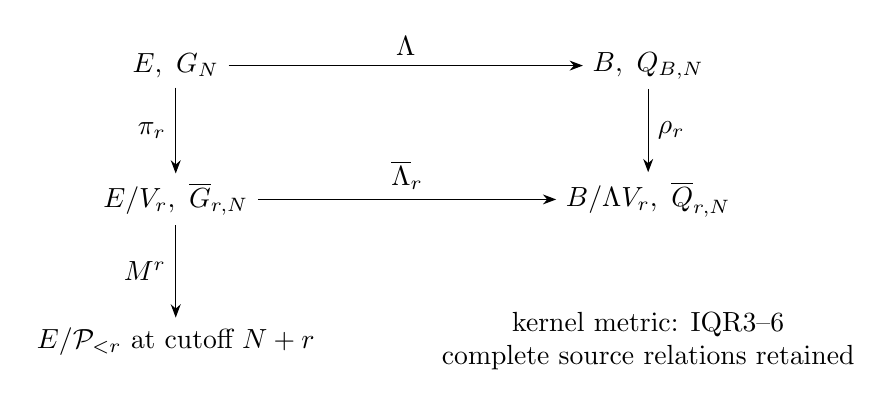
\begin{tikzpicture}[>=Stealth]
\node (e) at (0,2.8) {$E,\ G_N$};
\node (b) at (6,2.8) {$B,\ Q_{B,N}$};
\node (er) at (0,1.1) {$E/V_r,\ \overline G_{r,N}$};
\node (br) at (6,1.1) {$B/\Lambda V_r,\ \overline Q_{r,N}$};
\node (sh) at (0,-.7) {$E/\mathcal P_{<r}$ at cutoff $N+r$};
\draw[->] (e)--node[above]{$\Lambda$}(b);
\draw[->] (e)--node[left]{$\pi_r$}(er);
\draw[->] (b)--node[right]{$\rho_r$}(br);
\draw[->] (er)--node[above]{$\overline\Lambda_r$}(br);
\draw[->] (er)--node[left]{$M^r$}(sh);
\node[align=center] at (6,-.7) {kernel metric: IQR3--6\\
complete source relations retained};
\end{tikzpicture}
\caption{Exact quotient and shifted-source maps. The horizontal
map's degree-zero cohomology is the original kernel. The vertical
source map removes $V_r$; multiplication moves its target to the low
polynomial quotient with the displayed changed cutoff. Every norm is
the attained original norm, not an unweighted coefficient norm.}
\end{figure}

\begin{figure}[ht]\centering
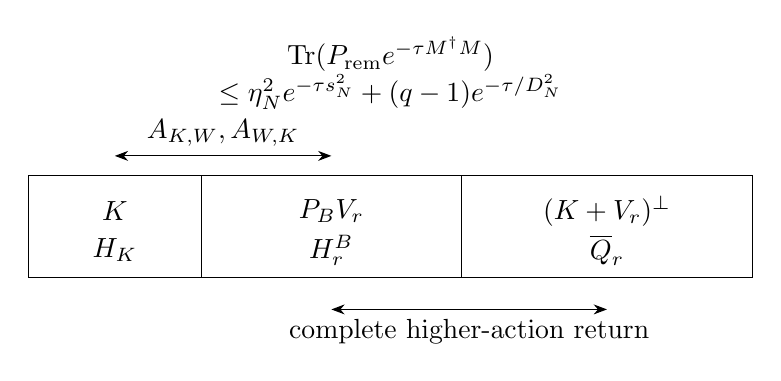
\begin{tikzpicture}[>=Stealth]
\draw (0,0) rectangle (2.2,1.3);
\draw (2.2,0) rectangle (5.5,1.3);
\draw (5.5,0) rectangle (9.2,1.3);
\node at (1.1,.85) {$K$};
\node at (3.85,.85) {$P_BV_r$};
\node at (7.35,.85) {$(K+V_r)^\perp$};
\node at (1.1,.35) {$H_K$};
\node at (3.85,.35) {$H^B_r$};
\node at (7.35,.35) {$\overline Q_r$};
\draw[<->] (1.1,1.55)--node[above]{$A_{K,W},A_{W,K}$}(3.85,1.55);
\draw[<->] (3.85,-.4)--node[below]{complete higher-action return}(7.35,-.4);
\node[align=center] at (4.6,2.6)
 {$\operatorname{Tr}(P_{\rm rem}e^{-\tau M^\dagger M})$\\
 $\le\eta_N^2e^{-\tau s_N^2}+(q-1)e^{-\tau/D_N^2}$};
\end{tikzpicture}
\caption{Exact orthogonal metric blocks, drawn schematically rather
than proportional to dimension. IQR8--10 bounds the residual heat;
IQR21 keeps both complex current cross blocks and the return through
the third block. A positive heat estimate is not used to assign a
complex-current sign.}
\end{figure}

\begin{thebibliography}{9}
\bibitem{IFH} Split-Zero research programme,
\href{https://github.com/KokunoYumeto/zeta-function-research-reader/blob/edd4008690952fb8568a01744e49ad7e180401e9/workbenches/splitzero-tandem/continuations/20260921-original-observation/INVERSE_FLAG_AND_RELATIVE_HEAT.tex}{The original observed inverse-power flag and its relative late heat},
IFH1--21, especially IFH10--21.
\bibitem{IVO} Independent finite derivation,
\href{https://github.com/KokunoYumeto/zeta-function-research-reader/blob/edd4008690952fb8568a01744e49ad7e180401e9/workbenches/splitzero-tandem/continuations/20260921-original-observation/INDEPENDENT_FINITE_OBSERVATION.tex}{IVO1--26, complete finite constants}.
\bibitem{ECL} Split-Zero research programme,
\href{https://github.com/KokunoYumeto/zeta-function-research-reader/blob/5992ad50c0f2a06921f1fcaded7b4e38097c0739/workbenches/splitzero-tandem/continuations/20260920-original-kernel-mixed-determinants/providers/09_INPUT_CUMULATIVE_PROOFS.tex#L28161}{The exact closed equilibrium coefficient, ECL1--17}.
Its full proof is retained in the accompanying cumulative source.
\bibitem{NP} Split-Zero research programme,
\href{https://github.com/KokunoYumeto/zeta-function-research-reader/blob/5992ad50c0f2a06921f1fcaded7b4e38097c0739/workbenches/splitzero-tandem/continuations/20260920-original-kernel-mixed-determinants/providers/09_INPUT_CUMULATIVE_PROOFS.tex#L124542}{NP18--19},
and \href{https://github.com/KokunoYumeto/zeta-function-research-reader/blob/5992ad50c0f2a06921f1fcaded7b4e38097c0739/workbenches/splitzero-tandem/continuations/20260920-original-kernel-mixed-determinants/providers/09_INPUT_CUMULATIVE_PROOFS.tex#L124713}{NP30--31, full proper-source minimum}.
\bibitem{NG} Split-Zero research programme,
\href{https://github.com/KokunoYumeto/zeta-function-research-reader/blob/5992ad50c0f2a06921f1fcaded7b4e38097c0739/workbenches/splitzero-tandem/continuations/20260920-original-kernel-mixed-determinants/providers/NATIVE_GAUSSIAN_TRANSFER.tex#L50}{NG2--3, full original source comparison and multiplication}.
\bibitem{Smallest} Supplied mathematical continuation,
\href{https://github.com/KokunoYumeto/zeta-function-research-reader/blob/0fd693c844aad9117e30ec447c59864a28af10f3/workbenches/splitzero-tandem/continuations/20260921-native-spectral-real-pair/003/NATIVE_SMALLEST_SINGULAR_PROOF.tex}{S1--45}, especially S12--16 and S39--45.
\bibitem{Profile} Supplied mathematical continuation,
\href{https://github.com/KokunoYumeto/zeta-function-research-reader/blob/0fd693c844aad9117e30ec447c59864a28af10f3/workbenches/splitzero-tandem/continuations/20260921-native-spectral-real-pair/003/RETAINED_PROFILE_PROOF.tex}{H1--9, full original outgoing profile}.
\bibitem{Mixed} Supplied mathematical continuation,
\href{https://github.com/KokunoYumeto/zeta-function-research-reader/blob/78ed538f7c00121ab66e9e8adbefc0612c118db8/workbenches/splitzero-tandem/continuations/20260921-mixed-family-proof-source/COMPLETE_MIXED_SOURCE_PROOFS.tex#L129}{Original-metric heat transitions and complete mixed-family control, H17--23},
and \href{https://github.com/KokunoYumeto/zeta-function-research-reader/blob/78ed538f7c00121ab66e9e8adbefc0612c118db8/workbenches/splitzero-tandem/continuations/20260921-mixed-family-proof-source/COMPLETE_MIXED_SOURCE_PROOFS.tex#L528}{C6--10}. The complete original text and TeX accompany this edition.
\bibitem{Stacks} The Stacks Project Authors,
\href{https://stacks.math.columbia.edu/tag/0115}{Tag 0115, acyclic complexes and quasi-isomorphisms};
original author source
\href{https://github.com/stacks/stacks-project/blob/a04446e57ec1fbc252a871afcec7752fb2807b14/homology.tex#L3057}{cochain homotopies}
and \href{https://github.com/stacks/stacks-project/blob/a04446e57ec1fbc252a871afcec7752fb2807b14/homology.tex#L3160}{the definition}.
The finite contraction is supplied explicitly in received equations
(15)--(18); the terminology is not a new general construction.
\bibitem{DLMF} T. H. Koornwinder, R. Wong, R. Koekoek,
R. F. Swarttouw, with W. P. Reinhardt, NIST DLMF Chapter 18,
\href{https://dlmf.nist.gov/18.22.E8}{Meixner--Pollaczek recurrence}
and \href{https://dlmf.nist.gov/18.23.E7}{generating function}.
The original Gamma mass and recurrence in S12--16 retain these
human-source conventions. Their complete specialized estimates
are proved in the cited programme sources.
\end{thebibliography}\end{document}
